\documentclass[a4paper,12pt]{article}
\usepackage{ctex}
\usepackage{amsmath}
\usepackage{graphicx}
\usepackage{geometry}
\usepackage{multirow}
\usepackage{float}
\usepackage{subcaption}
\usepackage{csvsimple}
\geometry{left=2.5cm,right=2.5cm,top=2.5cm,bottom=2.5cm}
\graphicspath{{figures/}{results/}}
\begin{document}
\begin{titlepage}
    \centering
    \vfill
    {\zihao{0}\bfseries 电子测试与实验技术\\[0.6em]实验报告\par}
    \vfill
    \vfill

    \begin{minipage}{0.72\textwidth}
        \zihao{-2}
        学\quad\quad 院：\underline{\makebox[7.5cm][l]{光学与电子信息学院}}\\[1.6em]
        班\quad\quad 级：\underline{\makebox[7.5cm][l]{光电信息科学与工程202409班}}\\[1.6em]
        姓\quad\quad 名：\underline{\makebox[7.5cm][l]{陈\quad 恪\quad 瑾}}\\[1.6em]
        学\quad\quad 号：\underline{\makebox[7.5cm][l]{U 2 0 2 4 1 3 9 2 5}}\\[1.6em]
        实验时间：\underline{\makebox[7.5cm][l]{2026 年 04 月 23 日}}
    \end{minipage}

    \vfill
    \vfill
\end{titlepage}

\setcounter{page}{1}



\section{实验名称}
正弦波产生和精密整流。

\section{实验目的}
\begin{enumerate}
    \item 了解集成运算放大器在振荡电路方面的作用。
    \item 掌握由集成运算放大器构成的桥式振荡电路的工作原理、震荡频率和输出幅度的测量方法。
    \item 研究负反馈强弱对振荡波形的影响。
    \item 学习用示波器测量正弦波的振荡频率、开环幅频特性和相频特性的方法。
    \item 学习用运算放大器构成精密全波整流电路的方法。
    \item 重点掌握精密全波整流电路输入、输出波形的测量和描绘方法。
\end{enumerate}

\section{实验元器件}
\begin{table}[H]
\centering
\caption{正弦波产生电路实验元器件}
\begin{tabular}{|c|c|c|}
\hline
类型         & 型号（参数） & 数量 \\
\hline
集成运算放大器 & LM324       & 1片  \\
\hline
电位器       & 100k$\Omega$ & 1只  \\
\hline
电阻         & 5.1k$\Omega$ & 2只  \\
\hline
电阻         & 10k$\Omega$  & 2只  \\
\hline
电阻         & 18k$\Omega$  & 2只  \\
\hline
二极管       & 2AP7         & 2只  \\
\hline
电容         & 0.033$\mu$F  & 2只  \\
\hline
\end{tabular}
\end{table}

\begin{table}[H]
\centering
\caption{精密全波整流电路实验元器件}
\begin{tabular}{|c|c|c|}
\hline
类型         & 型号（参数）   & 数量 \\
\hline
集成运算放大器 & LM324         & 1片  \\
\hline
电位器       & 100k$\Omega$  & 1只  \\
\hline
电阻         & 3.3k$\Omega$  & 1只  \\
\hline
电阻         & 10k$\Omega$   & 5只  \\
\hline
电阻         & 20k$\Omega$   & 1只  \\
\hline
二极管       & 2AP7          & 2只  \\
\hline
\end{tabular}
\end{table}


\section{实验原理}
\subsection{正弦波产生电路}
\subsubsection{参考电路}
RC 文氏电桥正弦波振荡电路如图所示，核心由运算放大器、RC 串并联选频网络、负反馈网络及稳幅二极管构成。
\begin{figure}[H]
    \centering
    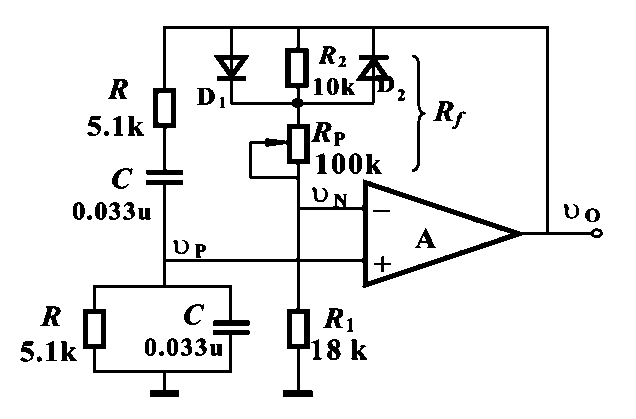
\includegraphics[width=0.72\textwidth]{figures/reference/9-1.png}
    \caption{正弦波产生电路实验参考电路}
    \label{fig:reference9_1}
\end{figure}

\subsubsection{实验原理}
图中 R、C 为串、并联选频网络，接于运算放大器的输出端与同相输入端之间，构成正反馈，以产生正弦自激振荡。其余部分是带有负反馈的同相放大电路，$R_1$、$R_2$、$R_P$ 构成负反馈网络，调节 $R_P$ 可改变负反馈的反馈系数，从而调节放大电路的电压增益，使其满足振荡的幅值条件。

二极管 $D_1$、$D_2$ 有利于正弦波的起振和稳定输出幅度，改善输出波形。当输出电压 $V_o$ 幅值很小时，$D_1$、$D_2$ 开路，等效电阻 $R_f$ 较大，电压增益
\[
A_{vf}=\frac{V_o}{V_p}=\frac{R_1+R_f}{R_1}
\]
较大，有利于起振；当输出幅值较大时，二极管导通，$R_f$ 减小，$A_{vf}$ 下降，幅值趋于稳定。

设 R、C 串并联网络中，并联阻抗为 $Z_1$，串联阻抗为 $Z_2$，振荡角频率为
\[
\omega_0=\frac{1}{RC}
\]
则
\[
Z_1=\frac{R}{1+j\omega RC},\quad Z_2=R+\frac{1}{j\omega C}
\]

正反馈系数为
\[
F_v=\frac{V_p}{V_{12}}=\frac{Z_1}{Z_1+Z_2}
=\frac{1}{3+j\left(\dfrac{\omega}{\omega_0}-\dfrac{\omega_0}{\omega}\right)}
\]

当 $\omega=\omega_0$ 时，反馈系数幅值最大，$F_v=1/3$，相角 $\varphi_f=0^\circ$，满足自激振荡相位条件。若此时负反馈放大电路增益大于 3，则满足 $A_{vf}F_v>1$ 的起振条件。电路起振后，受二极管非线性限制，增益由 $A_{vf}>3$ 过渡到 $A_{vf}=3$，达到幅值平衡。

\begin{figure}[H]
    \centering
    \begin{subfigure}{0.47\textwidth}
        \centering
        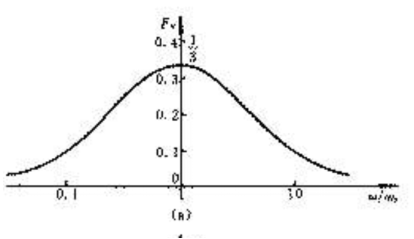
\includegraphics[width=\textwidth]{figures/reference/9-2.png}
        \caption{幅频相应曲线}
        \label{fig:A_f}
    \end{subfigure}
    \hfill
    \begin{subfigure}{0.47\textwidth}
        \centering
        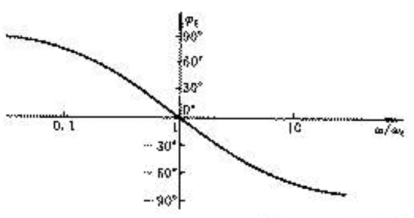
\includegraphics[width=\textwidth]{figures/reference/9-3.png}
        \caption{相频响应曲线}
        \label{fig:phi_f}
    \end{subfigure}
    \caption{串、并联选频网络的频率响应}
    \label{fig:A_or_phi_f}
\end{figure}

\subsubsection{注意事项}
\begin{enumerate}
    \item 安装电路时，应注意集成运算放大器各引脚的功能和二极管的极性。
    \item 调整电路时，应反复调电位器，使电路起振，且波形幅值最大且不失真。
    \item 测量振荡电路的开环相频特性时，注意相位差角 $\varphi_f$ 在 $f_0$ 前后会发生明显变化。
\end{enumerate}

\subsection{精密全波整流电路}
\subsubsection{实验原理}
由于二极管的伏安特性在小信号时处于截止或特性曲线的弯曲部分，所以一般利用二极管的单向导电性来组成整流电路，在小信号检波时，输出端将得不到原信号（或使原信号失真很大），常常出现交越失真。如果把二极管置于运算放大器组成的负反馈环路中，则能大大削弱这种影响，提高电路的精度。

\begin{figure}[H]
    \centering
    \begin{subfigure}{0.47\textwidth}
        \centering
        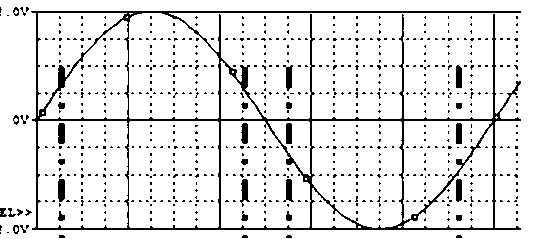
\includegraphics[width=\textwidth]{figures/reference/10-1.png}
        \caption{输入信号}
        \label{fig:reference10_1}
    \end{subfigure}
    \hfill
    \begin{subfigure}{0.47\textwidth}
        \centering
        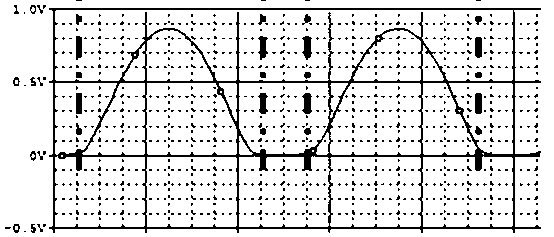
\includegraphics[width=\textwidth]{figures/reference/10-2.png}
        \caption{输出信号}
        \label{fig:reference10_2}
    \end{subfigure}
    \caption{交越失真示意图}
    \label{fig:reference10_1_and_10_2}
\end{figure}

\subsubsection{参考电路}
如图所示是反相输入精密全波整流电路。

\begin{figure}[H]
    \centering
    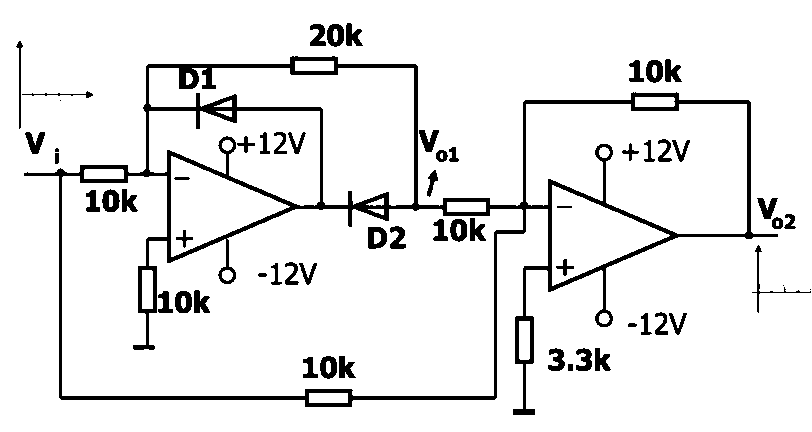
\includegraphics[width=0.72\textwidth]{figures/reference/10-3.png}
    \caption{精密全波整流电路实验参考电路}
    \label{fig:reference10_3}
\end{figure}

当输入电压 \( V_I>0 \) 时，二极管 \( D_1 \) 截止，\( D_2 \) 导通，\( A_1 \) 为反相比例运算电路，\( A_2 \) 为加法运算电路，可计算得到输出端电压为：
\[
V_{O1}=-\frac{20\,\text{k}\Omega}{10\,\text{k}\Omega}V_I=-2V_I
\]
\[
V_O=-\left( \frac{10\,\text{k}\Omega}{10\,\text{k}\Omega}V_{O1} \right)+\left( -\frac{10\,\text{k}\Omega}{10\,\text{k}\Omega}V_I \right)=V_I
\]

输入电压 \( V_I<0 \) 时，二极管 \( D_1 \) 导通，\( D_2 \) 截止，
\[
V_{O1}=0,\quad V_O=-V_I
\]

上述分析表明，该电路在输出端可得到单向电压，实现了全波整流。其电压传输特性及输入、输出电压波形如图所示。

\begin{figure}[H]
    \centering
    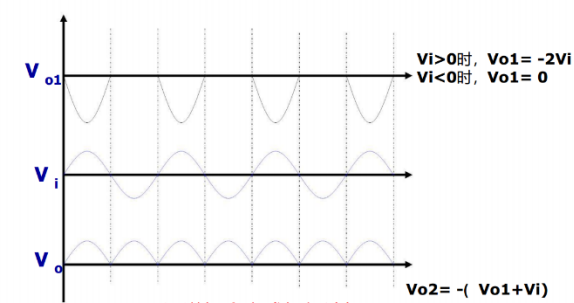
\includegraphics[width=0.72\textwidth]{figures/reference/10-4.png}
    \caption{电压传输特性及输入、输出电压波形}
    \label{fig:reference10_4}
\end{figure}

\subsubsection{注意事项}
整流的精度决定于 \( R_{f1} \)、\( R_{f2} \)、\( R_1 \)、\( R_2 \) 的匹配精度。


\section{硬件实验内容}
\subsection{正弦波产生电路}
\subsubsection{组装电路}
按照实验电路图在实验板上正确连接电路，检查接线无误后接通电源。

\subsubsection{观察输出波形}
将示波器接在振荡电路的输出端，观察输出波形 \( V_O \)。适当调节电位器 \( R_P \)，使电路产生振荡，观察负反馈强弱（即电压增益 \( A_{vf} \) 大小）对输出波形 \( V_O \) 的影响。

\subsubsection{测量输出电压峰-峰值和输出信号频率}
在输出波形 \( V_O \) 基本不失真的情况下，分别测量输出电压的峰-峰值和振荡频率 \( f_0 \)，并绘制波形图。

\subsubsection{测量开环幅频特性和相频特性}

\paragraph{幅频特性}
在实验电路图中将 a 点断开，从 1、2 两点间输入信号 \( V_{12} \)。为保持放大器工作状态不变，\( V_{12} \) 的幅值应与步骤 5.3 测得的输出电压峰-峰值保持一致。改变输入信号 \( V_{12} \) 的频率并保持幅值不变，分别测量对应的输出电压峰-峰值，记入实验数据表格。

\paragraph{相频特性}
在实验电路图中将 a 点断开，输入信号 \( V_{12} \)，改变输入信号频率，观测输出电压 \( V_O \) 与输入信号 \( V_{12} \) 之间的相位差，记入实验数据表格。


\subsection{精密全波整流电路}
\subsubsection{组装电路与调零}
按照图组装电路（电源电压为$\pm12\,\text{V}$），检查无误后，接通电源。进行电路调零。将输入端接地（使$V_I=0$），缓慢调节运放调零端的外接电位器，使输出电压为零。

\subsubsection{测量直流传输特性}
在输入端加正、负直流电压，分别测出$V_{O1}$、$V_{O1}'$和$V_O$，并画出$V_O$-$V_I$的传输特性曲线。

\subsubsection{观测交流输入波形}
输入正弦电压峰-峰值为4V、$f=1\,\text{kHz}$，观测并记录$V_I$、$V_{O1}$和$V_O$波形，标出它们的幅值和相位。注意：用$V_I$作为信号触发源。

\subsubsection{观测电压传输特性曲线}
直接用示波器的X-Y方式观察电压传输特性曲线（注意坐标原点的调节方法）。


\section{硬件实验结果分析}
\subsection{正弦波产生电路}
\subsubsection{实验插板图}
实验电路插板搭建如图所示（图略）。

\subsubsection{实验波形}
\paragraph{振荡波形}
示波器测得稳定正弦振荡波形，核心参数：
峰峰值 \( V_{pp}=3.480\,\text{V} \)，频率 \( f=733.1\,\text{Hz} \)，波形基本不失真。

\paragraph{相位差测量}
在谐振频率附近测量输入与输出信号相位差，谐振点相位差接近 \( 0^\circ \)，符合RC串并联选频网络特性。

\paragraph{振荡不起来的情况}
当负反馈过强、增益不足或接线错误时，电路无法满足起振条件，无振荡波形输出。

\paragraph{电压增益过大的情况}
电位器调节不当导致增益过高，波形严重失真，峰峰值可达 \( 15.20\,\text{V} \)，出现明显削波。

\subsubsection{实验数据}
调节 \( R_P \) 使振荡稳定且波形最大不失真，测得振荡频率 \( f_0=733\,\text{Hz} \)。保持 \( V_{12} \) 幅度不变，改变频率测得幅频与相频特性数据如下：

\begin{table}[H]
\centering
\caption{开环幅频特性与相频特性测量数据}
\begin{tabular}{|c|c|c|}
\hline
输入信号频率 \( f/\text{Hz} \) & 输出电压峰峰值 \( V_{pp}/\text{V} \) & 相位差 \( \varphi/^\circ \) \\
\hline
50    & 1.5   & 0 \\
\hline
70    & 0.76  & 79.2 \\
\hline
100   & 1.02  & 75.42 \\
\hline
200   & 1.4   & 67.95 \\
\hline
700   & 2.36  & 45.18 \\
\hline
\( f_0=733 \) & 3.44  & 2.022 \\
\hline
1200  & 3.44  & -17.39 \\
\hline
5000  & 3.28  & -66.93 \\
\hline
7000  & 1.14  & -70.59 \\
\hline
10000 & 0.84  & -73.73 \\
\hline
\end{tabular}
\end{table}

\paragraph{数据分析}
在谐振频率 \( f_0 \) 处输出幅度最大、相位差近似为 \( 0^\circ \)；频率偏离 \( f_0 \) 时输出幅度下降，相位差显著变化。实验结果与RC串并联选频网络理论特性基本一致。

\subsection{精密全波整流电路}
\subsubsection{实验插板图}
实验电路插板搭建如图所示（图略）。

\subsubsection{实验波形图}

\paragraph{半波整流}
其中黄色波形为输入信号，蓝色波形为半波整流所得波形。

\paragraph{全波整流}
其中黄色波形为输入信号，蓝色波形为精密全波整流后的波形。

\paragraph{示波器XY显示模式下传输特性曲线}
图示为传输特性曲线，因电路中可能存在某些接触不良的问题，噪声很大，存在一些不规则的“小颗粒”，但是主要特征还是清晰可见。课本上的图与实验所示图形基本一致，可知实验结果正确。

\subsubsection{实验数据}

\paragraph{原始数据}

\begin{table}[H]
\centering
\caption{精密全波整流电路直流输入输出测量数据}
\begin{tabular}{|c|c|c|c|c|c|c|c|c|}
\hline
输入直流电压 $V_I$/V & -5.0 & -0.7 & -0.5 & -0.3 & 0 & 0.3 & 0.5 & 5.0 \\
\hline
$V_{O1}'$/V & -9.4 & -770mV & -189mV & 188mV & 0 & 1.375V & 1.385V & 1.439V \\
\hline
$V_{O1}$/V & -8.6 & -206mV & 226mV & 625mV & 0 & 959mV & 987mV & 947mV \\
\hline
$V_O$/V & 5.767 & 1.105 & 0.730 & 0.498 & 0 & 0.537 & 0.743 & 5.929 \\
\hline
\end{tabular}
\end{table}

\paragraph{数据处理}
使用示波器的XY模式做出传输特性曲线如下图所示，测得数据不够平滑，虽有一定的误差，但是从形状上看，与示波器实际测得的波形近似，达到了实验的目的。

\section{实验总结}
\subsection{正弦波产生电路}
\subsubsection{问题及解决方案}
本次实验比较简单，实验过程顺利，未遇到明显故障与问题。

\subsubsection{操作技巧}
插装电路时，导线与引脚尽量剪短，避免布线过长，可提高电路稳定性，减少接触不良与干扰，便于一次性完成实验，也便于故障排查。


\subsubsection{问题及解决方案}
\begin{enumerate}
    \item 将信号发生器关闭，仅开启恒压直流源，将示波器直接与直流源相连，波形显示为规则的正弦波。
    
    \textbf{解决方法：} 地线没有接好，地线接触不良导致波形离谱，重新连接地线稳固后，奇怪的波形消失了。
    
    \item 整流后的波形出现晃动和变形，与上一个问题一样，是地线接触不良导致，重新连接后就解决了。
\end{enumerate}

\subsection{精密全波整流电路}
\subsubsection{实验小结}
本次实验对我来说又是一个全新的挑战，难度比上一个实验大了一些，第一个实验没有遇到什么问题，但是这个第二个实验出了一些诡异的问题，比如去掉输入信号后，示波器依然有规整的正弦波，解决之后恍然大悟，增长了我的见识，提高了我的动手能力和分析问题的能力，是很有收获的一次实验。


\subsection{心得体会}
通过本次实验，问题定位与排查能力得到进一步提升，面包板搭建与调试熟练度明显提高，同时也更加熟悉示波器在波形观察与参数测量中的使用方法。


\section{思考题}
\subsection{正弦波产生电路}
\begin{enumerate}
    \item 若想改变本实验电路的振荡频率，需要调节电路中的哪些元件？

    \textbf{解：} 根据自激振荡的相位条件，电路的频率应满足
    \[
    \omega=\omega_0=\frac{1}{RC}
    \]
    故需要调节选频网络中的电阻 \(R\) 和电容 \(C\) 以改变电路振荡频率。

    \item 分析电路调节输出电压幅度的原理，说明该电路中调整哪个元件可以改变输出电压 \(V_O\) 的幅度？

    \textbf{解：} 电路通过调节电位器 \(R_P\) 来改变电路的反馈系数，从而调节输出电压幅度。

    \item 试说明用示波器测量频率有哪几种常用方法？

    \textbf{解：} 第一，可以通过示波器的 measure 功能，选择测量的内容，自动测量波形的频率；

    第二，通过示波器的光标（cursor）功能，测量波形的周期，取倒数即为所测信号的频率。
\end{enumerate}

\subsection{精密全波整流电路}
\begin{enumerate}
    \item 如果本实验所选的电阻不匹配，则传输特性会怎么样？

    \textbf{解：} 本次实验所用的电路，其整流精度取决于电阻 \(R_{f1}\)、\(R_1\)、\(R_{f2}\)、\(R_2\) 的匹配精度。如果这四个电阻不能匹配，则得到的电路传输特性曲线在第一、第二象限的曲线斜率就不为 \(+1\)、\(-1\)，而有可能为其他的值。

    \item 如果运算放大器的零漂很大，则 \(V_O\) 波形会怎样？

    \textbf{解：} 在输入为零的时候，输出不为0即为零漂。若零漂很大，则输出信号的波形会出现抖动，在输入信号接近0处的波形会出现一定幅度的失真。
\end{enumerate}

\end{document}